\documentclass{beamer}
\usepackage{listings}
%
% Sunumunuzun nasıl görüneceğini seçin
%
% Daha fazla renk ve yazıtipi temaları için aşağıdaki adrese bakılabilir
% http://deic.uab.es/~iblanes/beamer_gallery/index_by_theme.html
%
\mode<presentation>
{
  \usetheme{Darmstadt}      % or try Darmstadt, Madrid, Warsaw, ...
  \usecolortheme{default} % or try albatross, beaver, crane, ...
  \usefonttheme{default}  % or try serif, structurebold, ...
  \setbeamertemplate{navigation symbols}{}
  \setbeamertemplate{caption}[numbered]
} 
\usepackage{graphics}
\usepackage{caption}
\usepackage{graphicx}
\usepackage{refstyle}
\usepackage[utf8]{inputenc} % Türkçe karakterler
\usepackage[T1]{fontenc} % Türkçe heceleme için
\usepackage[turkish,shorthands=:!]{babel} % Türkçe bölüm, şekil, tablo vb. isimler
\usepackage{minted} % Kaynak kodları gösterebilmek için kullanılır. Python pygments kütüphanesine ihtiyaç duyar.
\usepackage{hyperref} % Referanslara tıklayarak geçiş yapmayı sağlar.

\title[Bilgisayar Grafikleri]{Bilgisayar Grafikleri} % Örn: Yapay Zeka
\author[M.B. \& Ç.Ö.\& C.P.]{Mert Balkan\inst{1} \and Çağan Özkan \inst{2} \and Ceren Parmaksız \inst{3}} %Öğrenci isimleri bu kısıma girilecek
\institute[Bilgisayar Müh.]{\inst{1} 20253508 \and \inst{2} 21253071\inst{3} 20253081} 
\date{11.05.2022} % Bu kısma sunum tarihi girilecek (09.02.2018 gibi)

\begin{document}

\begin{frame}
  \titlepage
\end{frame}

% Anahat kısmını görüntülemek için aşağıdaki açıklama satırlarını kaldırın.
\begin{frame}{Outline}
  \tableofcontents
\end{frame}

\section{Bilgisayar Grafikleri Nedir?}
\section{Bilgisayar Grafiklerinin Tarihi}
\section{Bilgisayar Grafiklerinin Kullanım Alanları}
\section{OpenGL'de Örnek Bir Üçgen Çizimi}


\begin{frame}{Bilgisayar Grafikleri Nedir?}
\begin{itemize}
  \item Bilgisayar grafikleri, bilgisayarların ve \texttt{özel bir grafik donanımı ve yazılımının}  yardımıyla bir bilgisayar tarafından görüntü verisinin temsilini kullanarak oluşturulmuş grafiklerdir.
  \item Bilgisayarların etkileşimi ve anlaşılması ve verinin yorumlanması bilgisayar grafikleri sayesinde oldukça kolaylaşmıştır \cite{wikipedia}
\end{itemize}

\vskip 1cm %1 cm dikey boşluk bırakır

\begin{block}{Grafik Programlamda Kullanılan Bazı API Örnekleri}
DirectX, OpenGL, Vulkan API
\end{block}

\end{frame}


\begin{frame}{1950'li Yıllar}
\begin{itemize}
\item Ben Laposky'nin, osiloskopu kullanarak ilk kez bilgisayar grafiklerini kullanması 
\item MIT'de "The Whirlwind" isimli bilgisayar ilk kez gerçek zamanlı veriyi görsel bir şekilde gösterbiliyordu.
\item Light Pen icat edildi.
\end{itemize}
\begin{figure}
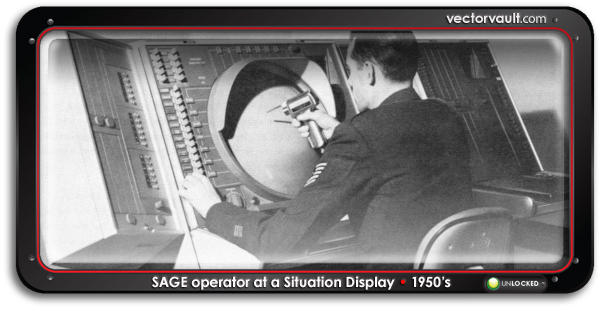
\includegraphics[width=0.4\textwidth]{artist.jpg} 
\caption{}
\end{figure}
\end{frame}

\begin{frame}[fragile]{1960'lı Yıllar}
\begin{itemize}
\item Osiloskopun yardımı ile "Spacewar" çıktı.
\item Ivan Sutherland bilgisayarda çizim yapabilen ilk yazılım olan SketchPad'i çıkardı.
\item Doug Engelbart mouse'yi icat etti.
\end{itemize}
\begin{columns}
\begin{column}{0.3\textwidth}
\begin{figure}
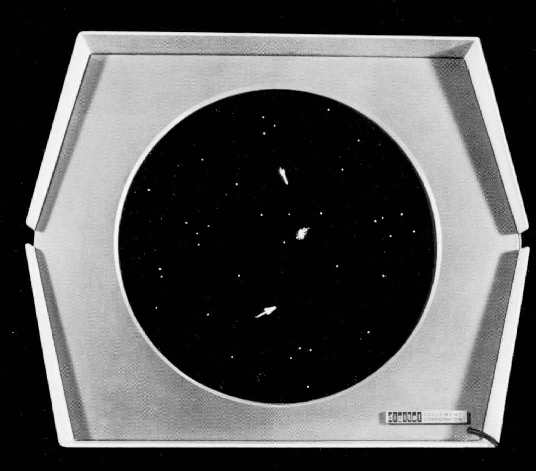
\includegraphics[width=\textwidth]{spacewar.jpg}
\caption{Spacewar}
\end{figure}
\end{column}
\begin{column}{0.4\textwidth}
\begin{figure}
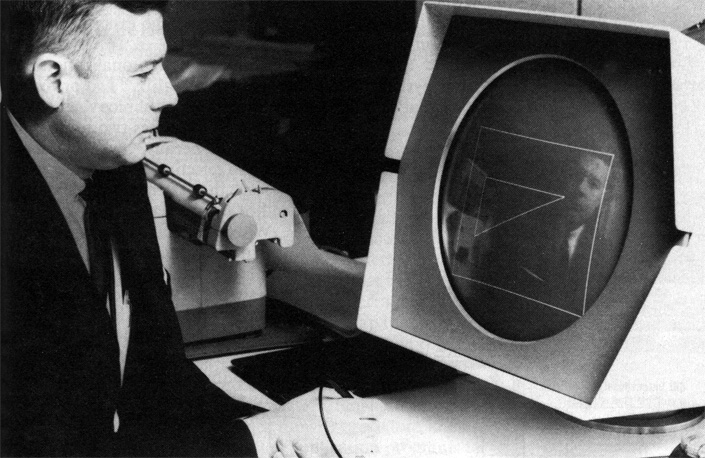
\includegraphics[width=\textwidth]{ıvansutherland.jpg}
\caption{SketchPad}
\end{figure}
\end{column}
\end{columns}
\end{frame}

\begin{frame}[fragile]{1960'lı Yıllar}
\begin{itemize}
\item Jack Bresenham çizgi çizebilen bir algoritma yazmıştır.
\item Ivan Sutherland görüntüyü gözümüze getirmiştir.
\item 1968'de Intel kurulmuştur.
\end{itemize}
\begin{columns}
\begin{column}{0.3\textwidth}
\begin{figure}
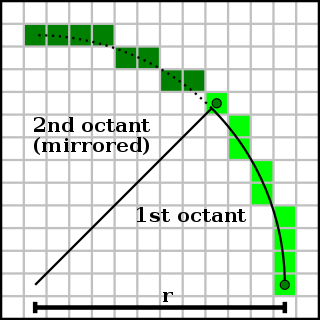
\includegraphics[width=\textwidth]{Bresenham_circle.svg.png}
\caption{Bresenham Çemberi}
\end{figure}
\end{column}
\begin{column}{0.4\textwidth}
\begin{figure}
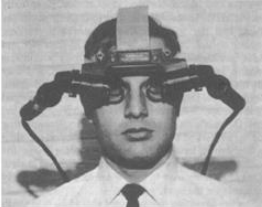
\includegraphics[width=\textwidth]{vr.PNG}
\caption{Kafaya Takılan Görüntüleme Cihazı }
\end{figure}
\end{column}
\end{columns}
\end{frame}

\begin{frame}{1970'li Yıllar}
\begin{itemize}
\item CADD(Computer-Aided Drafting and Design) 1970'te 25 milyon \$'a ulaştı.
\item Nolan Kay Bushnell "Pong" ilk arcade oyunu çıkardı.
\item CT scanner ve Raster Graphics çıktı.
\item Görüntüye sahip ilk kişisel bilgisayar Apple 2 çıktı.
\end{itemize}
\begin{columns}
\begin{column}{0.4\textwidth}
\begin{figure}
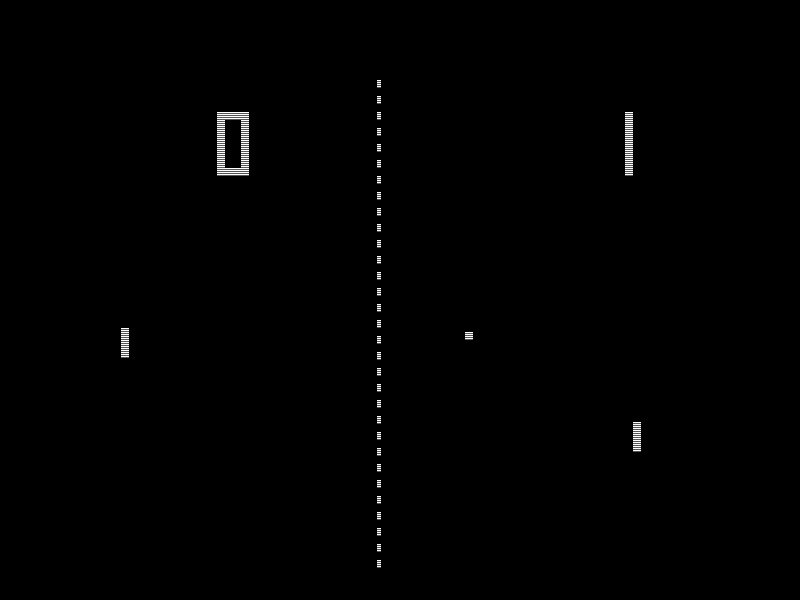
\includegraphics[width=\textwidth]{Pong.png}
\caption{Pong}
\end{figure}
\end{column}
\begin{column}{0.4\textwidth}
\begin{figure}
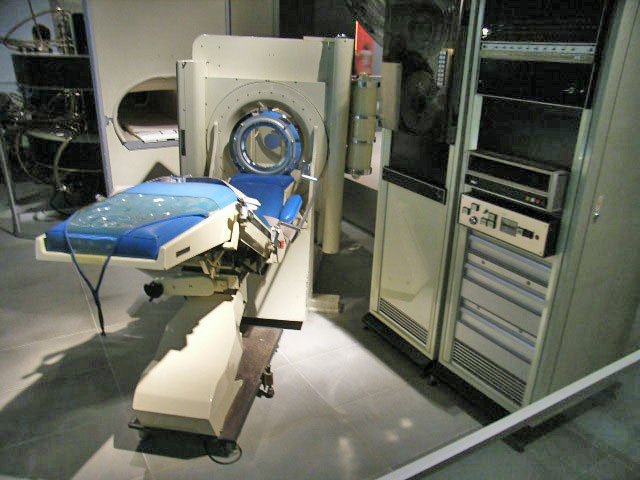
\includegraphics[width=\textwidth]{Emi1010.jpg}
\caption{CT scanner}
\end{figure}
\end{column}
\end{columns}
\end{frame}

\begin{frame}{1970'li Yıllar}
\begin{itemize}
\item Bu dönemde bir sürü "shading" tekniği ortaya çıkmıştır. Gouraud,Phong vb.
\item 1970'lerin sonunda CADD'ın market fiyatı 1 milyar \$'a ulaşmıştır. 
\begin{columns}
\begin{column}{0.4\textwidth}
\begin{figure}
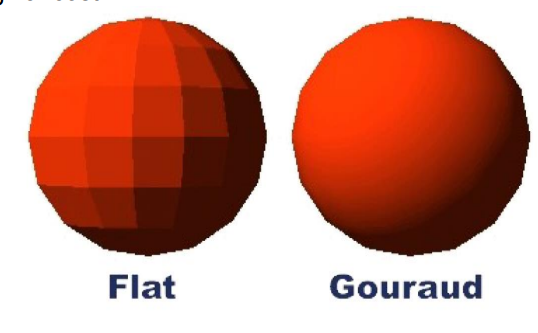
\includegraphics[width=\textwidth]{Gouraud.PNG}
\caption{Gouraud}
\end{figure}
\end{column}
\begin{column}{0.4\textwidth}
\begin{figure}
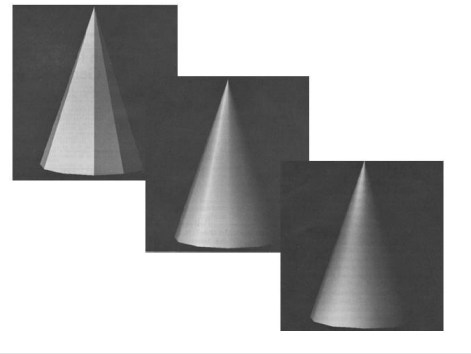
\includegraphics[width=\textwidth]{Phong.PNG}
\caption{Phong}
\end{figure}
\end{column}
\end{columns}
\end{itemize}
\end{frame}

\begin{frame}{1980'li Yıllar}
\begin{itemize}
\item Bu yıllarda Bilgisayar Grafikleri film sektörüne damgasını vurmuştur.
\item CGI yani "Computer Generated Imagery" ilk kez Disney'in "Tron" isimli filminde yer almıştır.

\begin{figure}
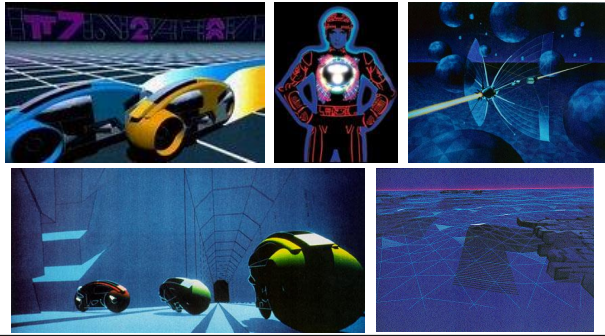
\includegraphics[width=0.6\textwidth]{tron.png}
\caption{Tron}
\end{figure}
\end{itemize}
\end{frame}

\begin{frame}{1980'li Yıllar}
\begin{itemize}
\item  Bu yıllar oyun sektörü için Altın Çağdır.
\end{itemize}
\begin{figure}
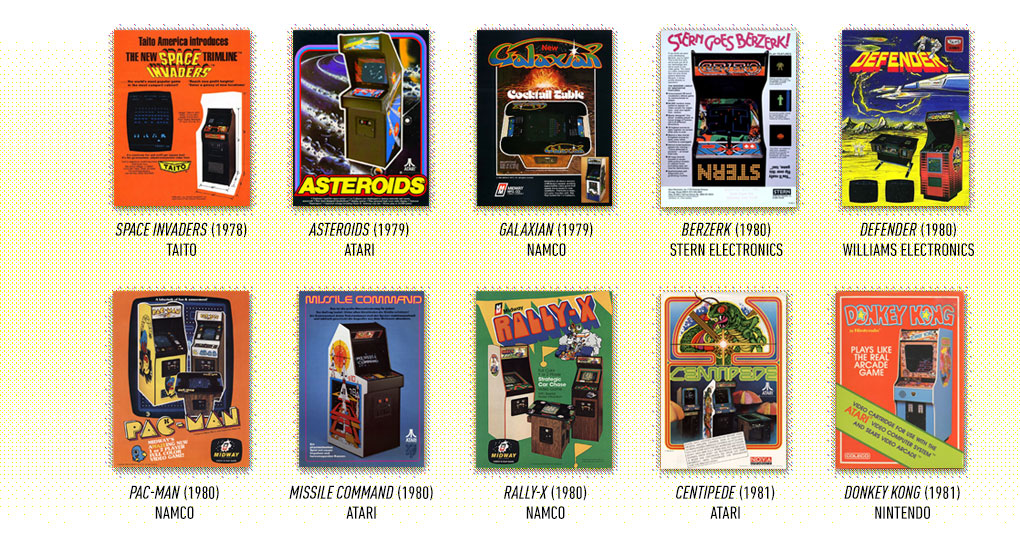
\includegraphics[width=0.8\textwidth]{arcade-timeline3.jpg}
\caption{Arcade oyunları}
\end{figure}
\end{frame}

\begin{frame}{1990'li Yıllar}
\begin{itemize}
\item Open Graphics Library (OpenGL) cross-platform API'si çıkmıştır.
\item Şu an çok popüler olan Nvidia çıkmıştır.
\item 3D modellemenin popülerleşmesi ile video oyunları hiç olmadığı kadar popüler olmuştur.
\item Toy Story 3, tamamı CGI olan ilk animasyon 1995'te çıkmıştır.
\end{itemize}
\begin{columns}
\begin{column}{0.4\textwidth}
\begin{figure}
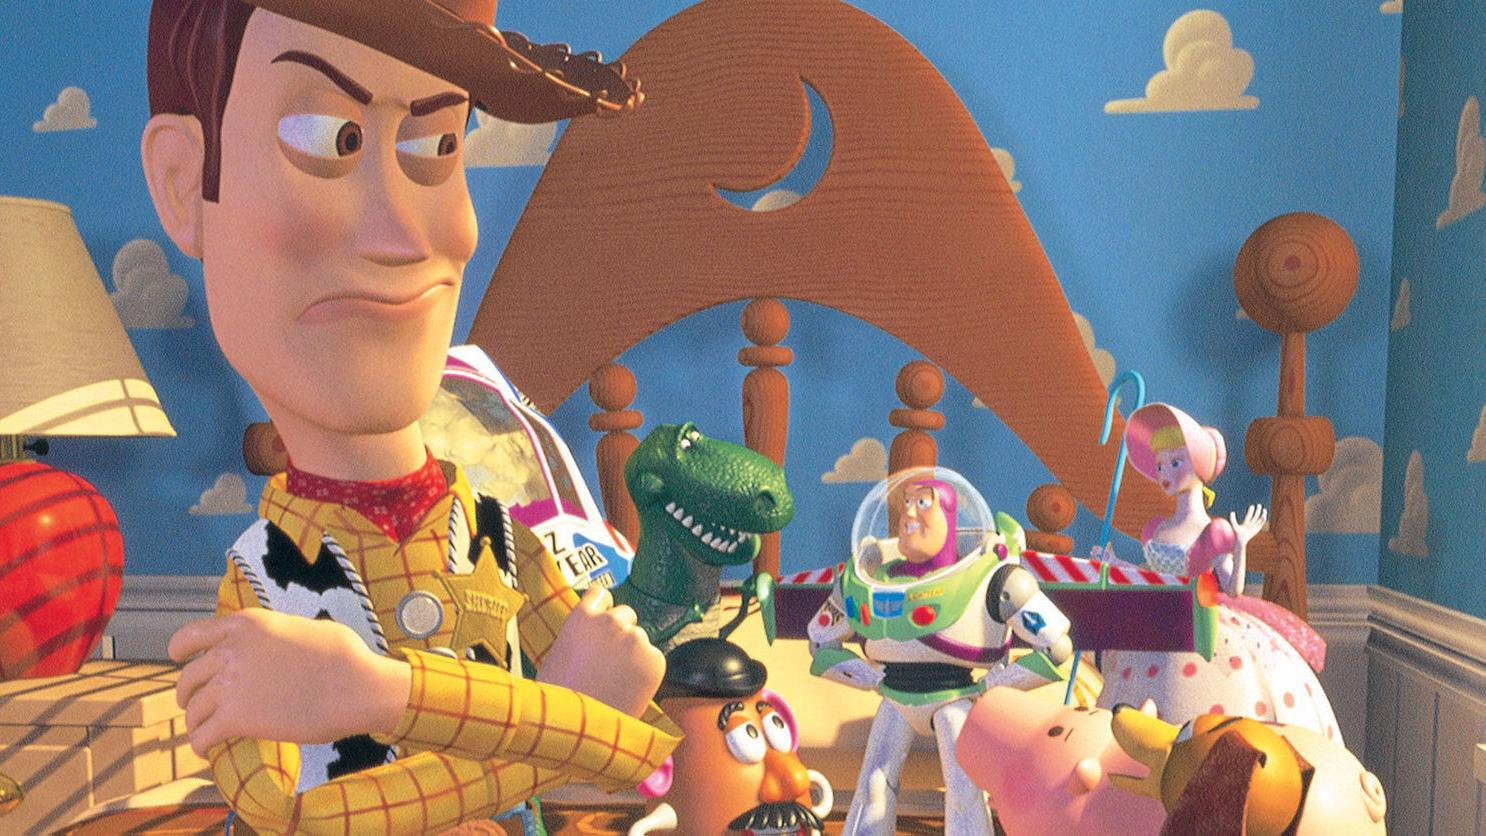
\includegraphics[width=\textwidth]{toystory.jpg}
\caption{Toy Story(1995)}
\end{figure}
\end{column}
\begin{column}{0.4\textwidth}
\begin{figure}
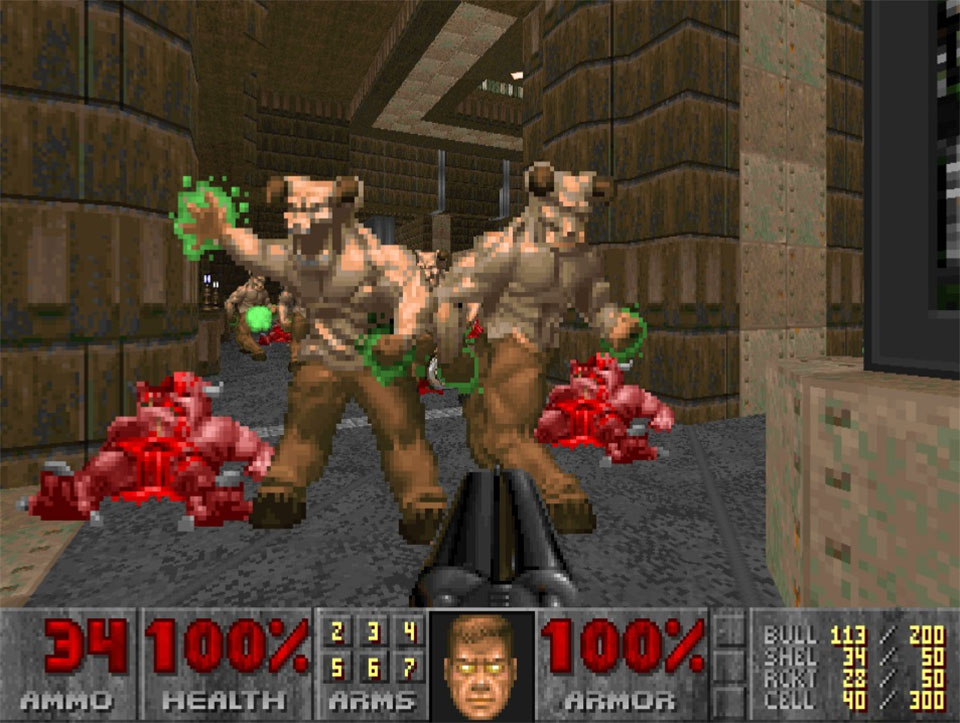
\includegraphics[width=\textwidth]{doom.jpg}
\caption{Doom (1993)}
\end{figure}
\end{column}
\end{columns}
\end{frame}

\begin{frame}{2000 ve Sonrası}
\begin{itemize}
\item Oyun konsolları çıkmıştır.
\item Nvidia ve Unreal Engine popülerleşmiştir.
\item Her filme CGI kolayca yerleştirilebilir.
\item Gelişmeler takip edilemeyecek kadar hızlanmıştır.
\end{itemize}
\begin{columns}
\begin{column}{0.3\textwidth}
\begin{figure}
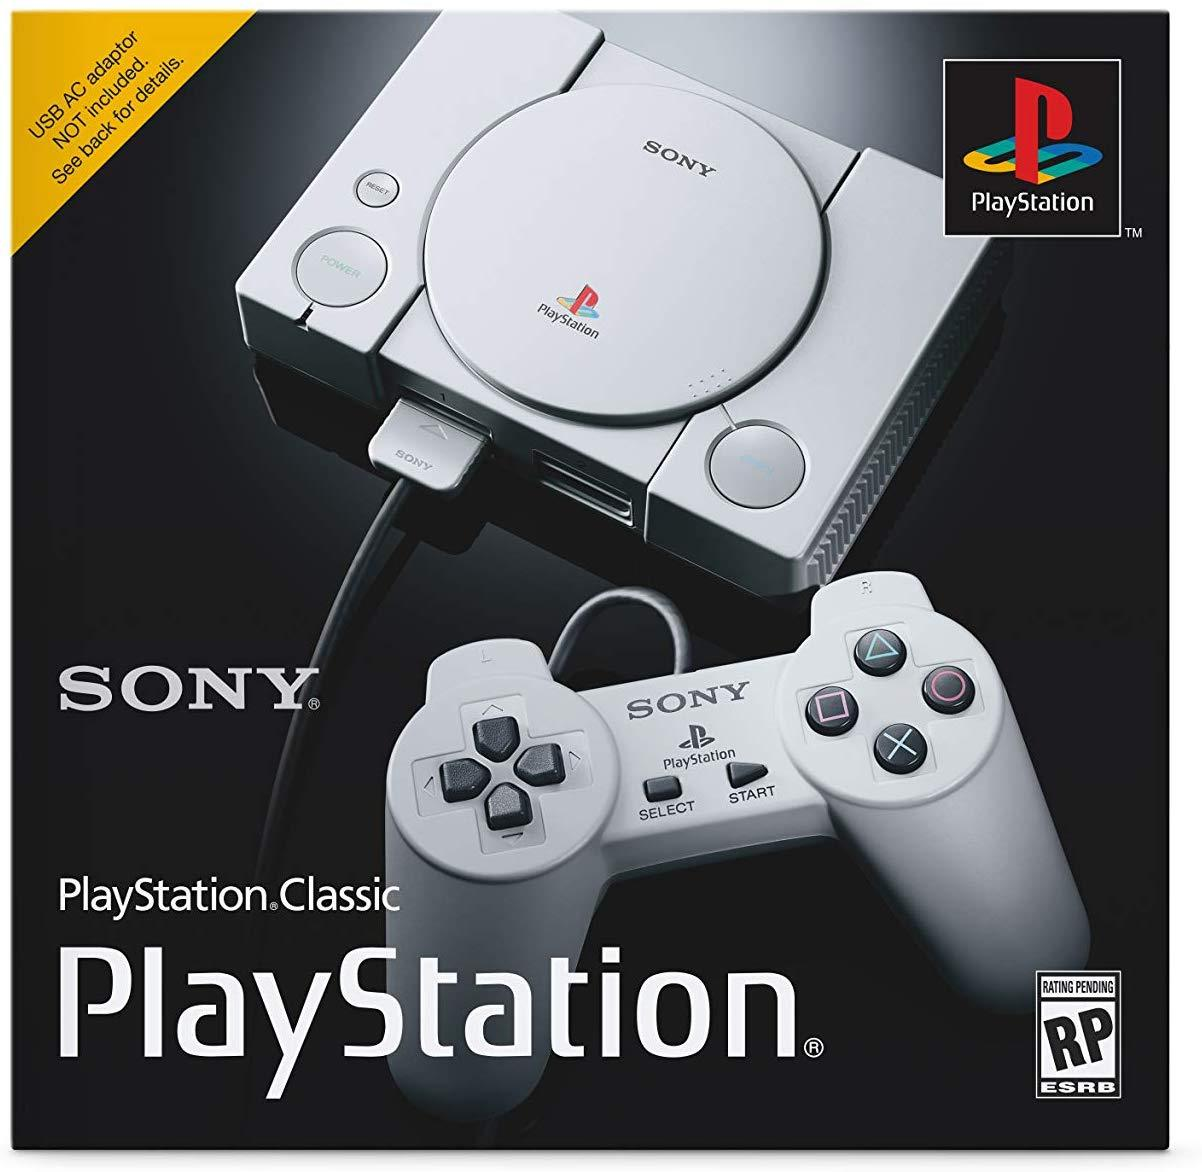
\includegraphics[width=\textwidth]{ps.jpg}
\caption{İlk Playstation}
\end{figure}
\end{column}
\begin{column}{0.5\textwidth}
\begin{figure}
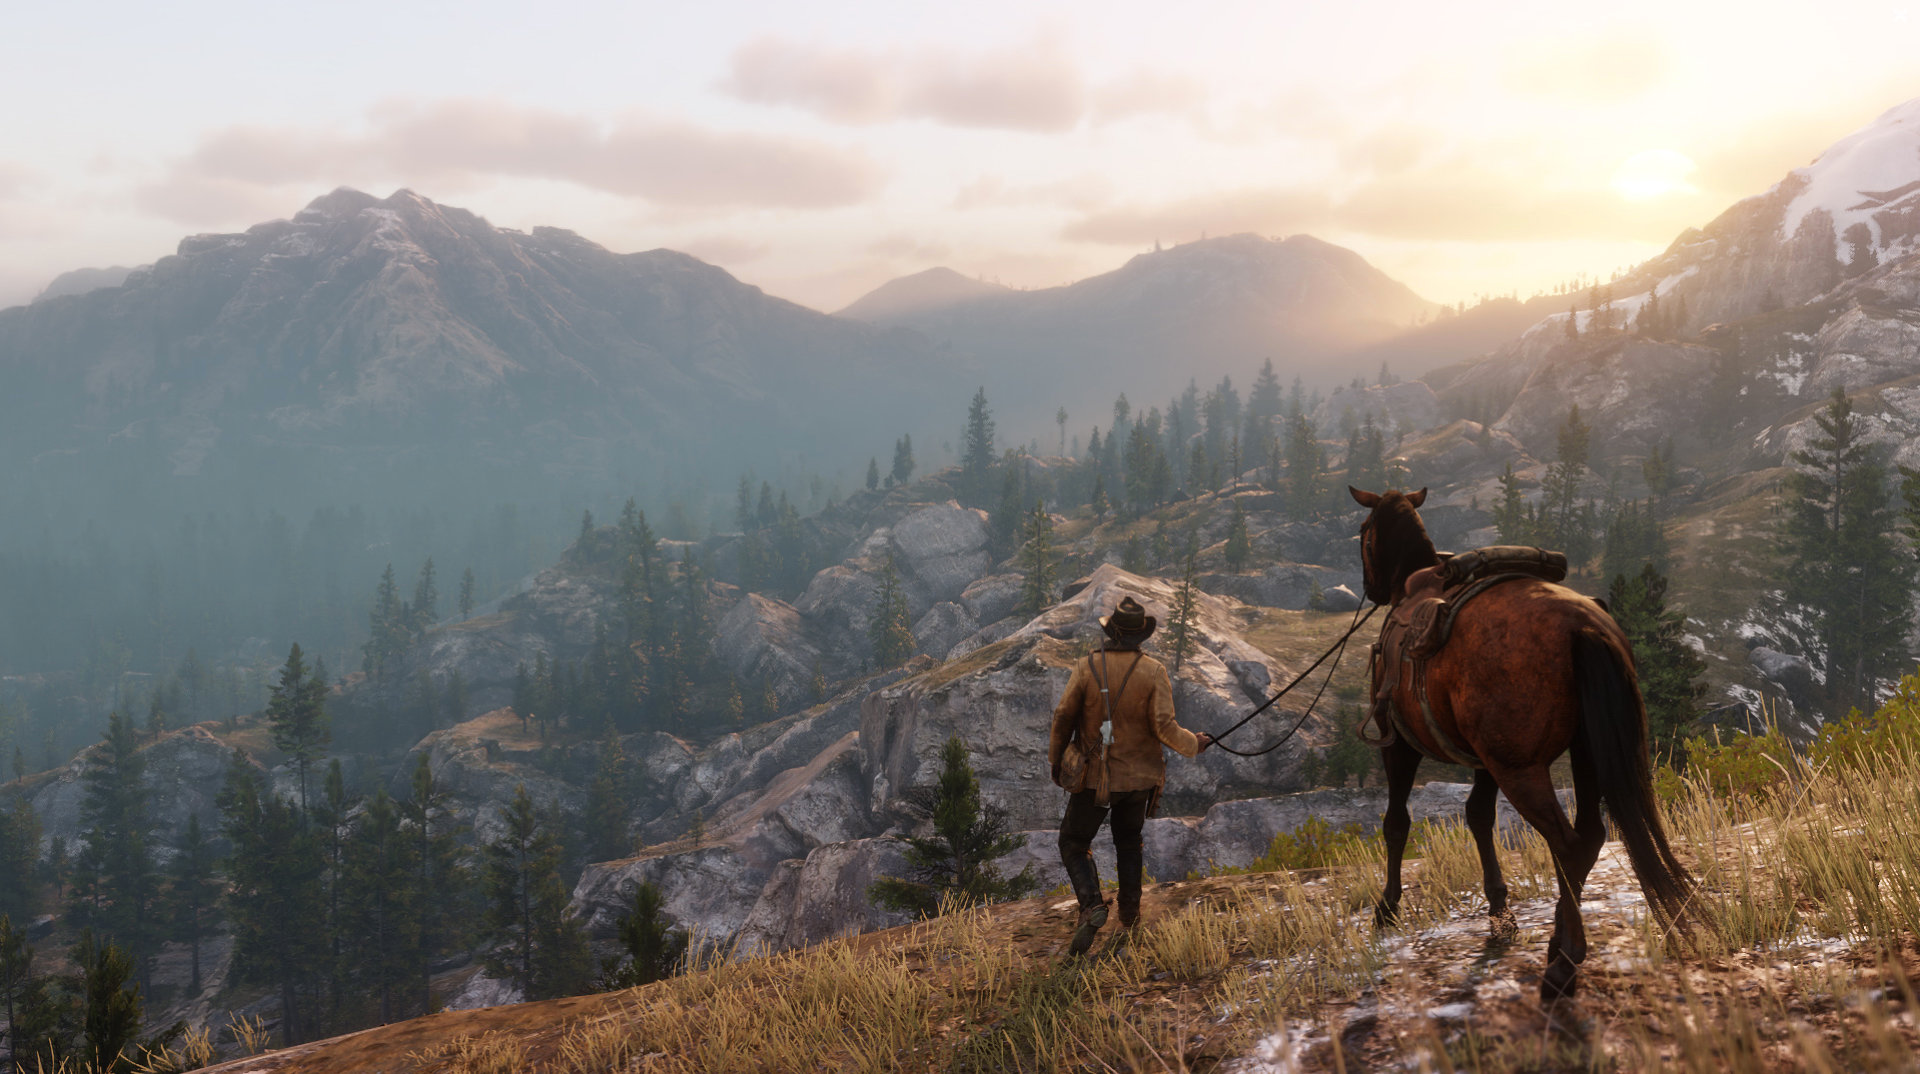
\includegraphics[width=\textwidth]{rdr2.jpg}
\caption{Red Dead Redemption}
\end{figure}
\end{column}
\end{columns}
\end{frame}




\begin{frame}{Bilgisayar Grafikleri Kullanım Alanları}
\begin{itemize}
    \item Gerçek Zamanlı 3 Boyutlu Canlandırma
    \item Resim işleme
    \item Tıbbi Görüntüleme
    \item Bilimsel Görselleştirme
    \item Animasyon (TV, filmler, reklamlar)
    \item Oyunlar
\end{itemize}
    
\end{frame}

\begin{frame}{Gerçek Zamanlı 3 Boyutlu Canlandırma}
\begin{itemize}
    \item Gerçek zamanlı 3B (3D) canlandırma, dijital bilgisayarlar üzerinde çalışan özel yazılımlar yardımıyla bir objenin geometrik bilgisi ve yüzey dokusu ile sürekli olarak canlandırılmasıdır. Bu canlandırma bilgisayar oyunlarının temelini oluşturur. Ayrıca 3B canlandırma; sağlık, mühendislik, askeri projeler vb. pek çok farklı alanda kullanılmaktadır.\cite{ebergi}
\end{itemize}
\begin{figure}
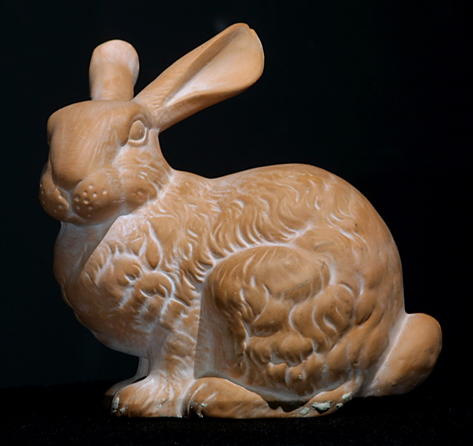
\includegraphics[width=0.4\textwidth]{3btest.PNG}
\caption{}
\end{figure}
    
\end{frame}

\begin{frame}{Resim İşleme}
\begin{itemize}
    \item Genelde 2Boyutlu resimler veya animasyon çerçeveleri üzerinde çeşitli işlemler olarak tanımlanabilir. Resim işlemenin de kullanım alanları çok çeşitlidir. Örnek vermek gerekirse bir görüntü üzerinde bir objenin yerinin tanımlanması çeşitli resim işleme algoritmaları ile yapılır. Aşağıdaki resim bir bilgisayar tarafından üretilmiştir.\cite{ebergi}
    
\end{itemize}
\begin{figure}
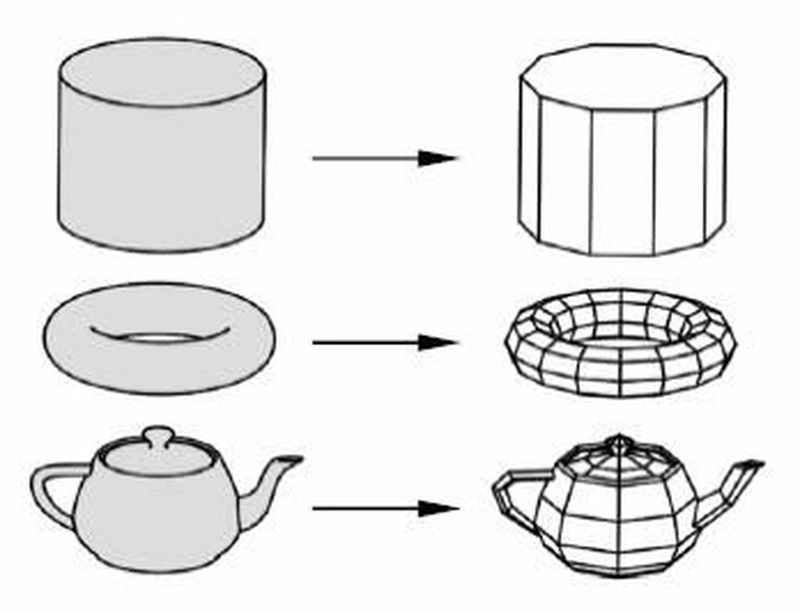
\includegraphics[width=0.4\textwidth]{resimisleme.jpg}
\caption{resim işleme}
\end{figure}
    
\end{frame}

\begin{frame}{Tıbbi Görüntüleme}
\begin{itemize}

    
    \item Bilgisayar grafiklerinin hayat kurtarmada önemli bir rol oynadığı söylenebilir.
Uygulama yelpazesi, tedaviye kadar öğretme ve tanılama araçlarından
oluşmaktadır.
    \item Işın izleme , bir görüntü düzlemindeki pikseller boyunca ışığın yolunu izleyerek bir görüntü oluşturmak için görüntü düzeni algoritmaları ailesinden bir tekniktir 
    \cite{omercetin}
\end{itemize}

\begin{figure}
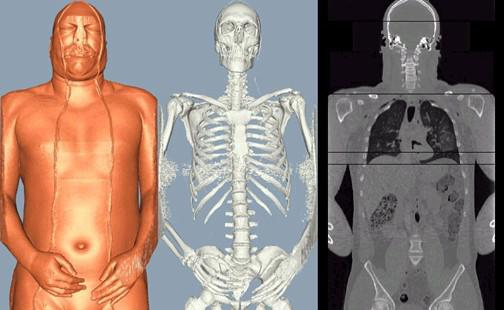
\includegraphics[width=0.4\textwidth]{img39.jpg}
\caption{}
\end{figure}
    
\end{frame}

\begin{frame}{Bilimsel görselleştirme}
\begin{itemize}
     \item Bilimsel görselleştirme bazı kavramları anlamak için soyut şeyleri görselleştiri.
    \item Matematikçiler soyut ve yüksek
boyutlu fonksiyon ve uzayları keşfetmek için bilgisayar grafiklerini kullanırlar.
Fizikçiler ölçek sınırlarını aşmak için bilgisayar grafiklerini kullanabilirler.
Bununla beraber hem mikroskobik hem de makroskobik dünyaları
keşfedebilirler.\cite{bilimselgorsellestirme}
   

\end{itemize}
\begin{figure}
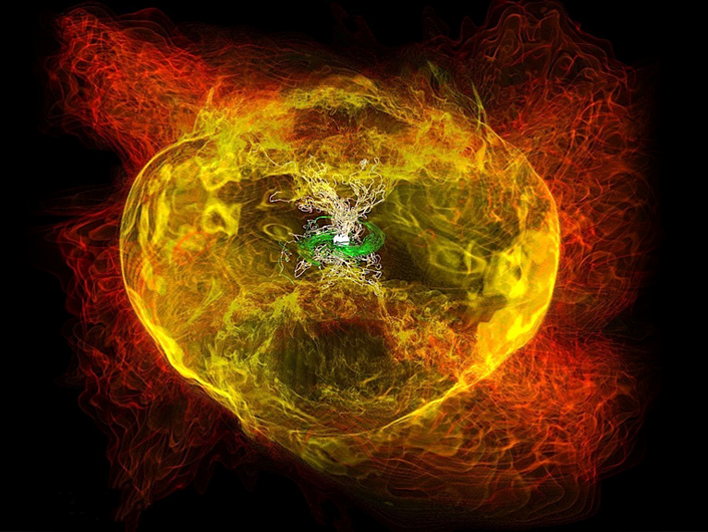
\includegraphics[width=0.3\textwidth]{görselleştirme.PNG}
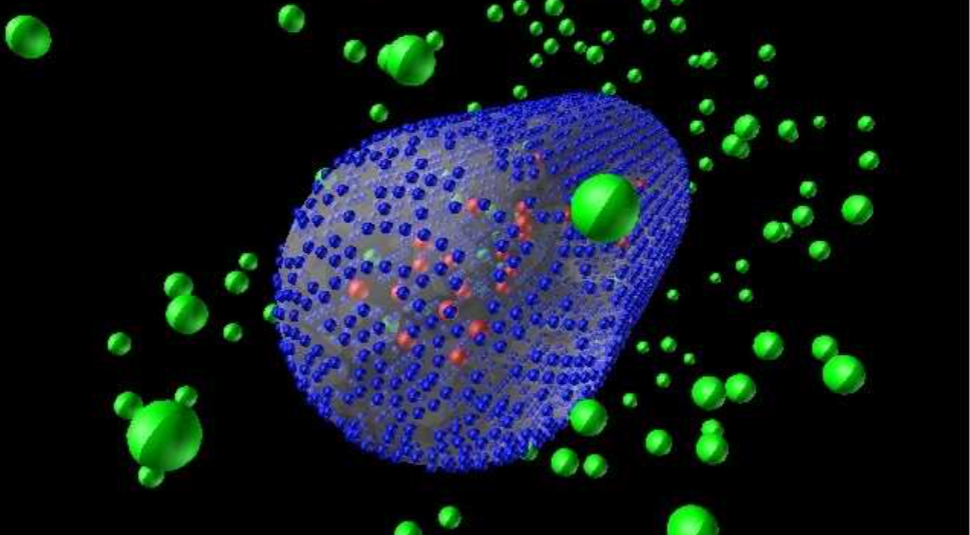
\includegraphics[width=0.3\textwidth]{bilimselgörsel.PNG}
\caption{2 nötron yıldızının çrpışması ve organizmalar}



\end{figure}

    
\end{frame}

\begin{frame}{Animasyon (TV, filmler, reklamlar)}
\begin{itemize}
    \item Bilgisayar animasyonu , bilgisayarları kullanarak hareketli görüntüler oluşturma sanatıdır .
    \item Animasyon elde etmek için birden fazla yöntem mevcuttur; animasyon yapılacak öznitelik başına her biri belirli bir zamanda bir değer depolayan ana karelerin oluşturulmasına ve düzenlenmesine dayanır . 2D/3D grafik yazılımı, her bir ana kare ile değişecek ve zamanla eşlenen bir değerin düzenlenebilir bir eğrisini yaratacak ve bu da animasyonla sonuçlanacaktır.\cite{omercetin}
    \item 
\end{itemize}

\begin{figure}
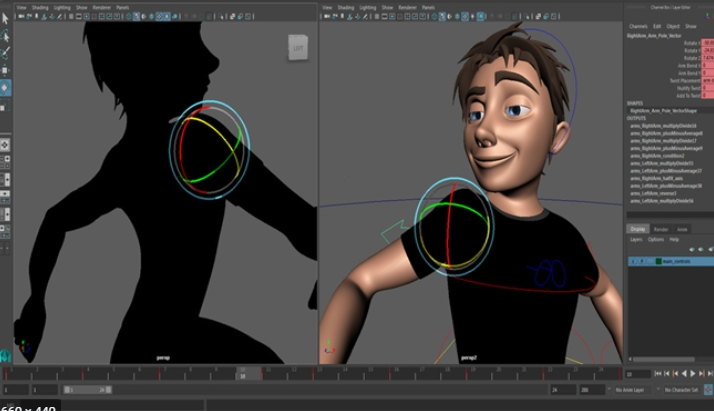
\includegraphics[width=0.4\textwidth]{animasyon.PNG}
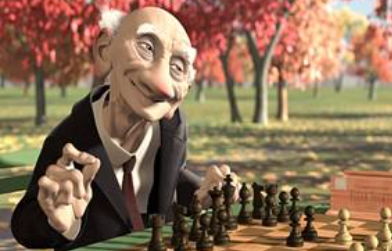
\includegraphics[width=0.4\textwidth]{animasyon2.PNG}
\caption{3D animasyon}
\end{figure}
    
\end{frame}

\begin{frame}{Oyunlar}
\begin{itemize}
    \item Oyunlar bilgisayar grafiklerinde önemli bir itici güçtür
    \item Daha çok 3D modelleme oyunların yapımında büyük bir yer kaplar bunun yanında gölgeleme,hacim oluşturma gibi birçok teknikten yararlanılarak oyunlar oluşturulur.
\end{itemize}

\begin{figure}
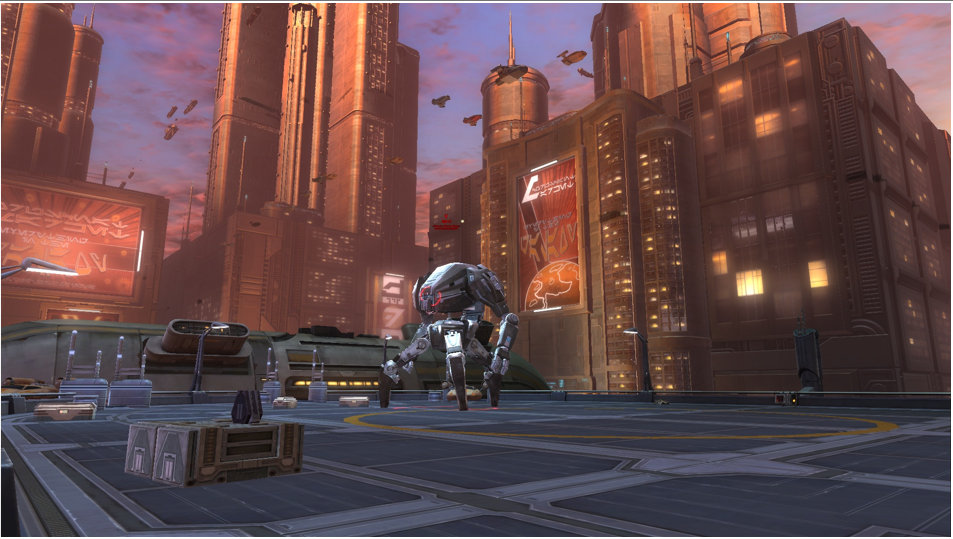
\includegraphics[width=0.4\textwidth]{oyunlar.PNG}
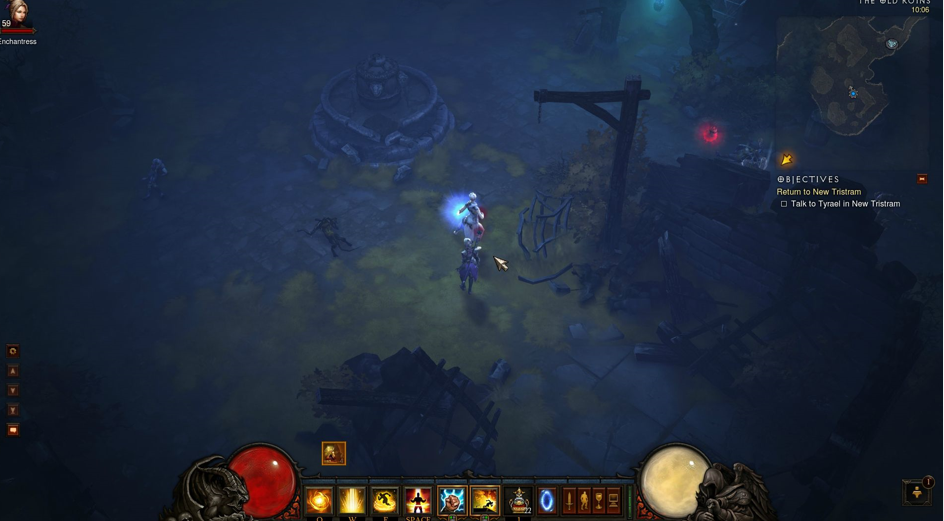
\includegraphics[width=0.4\textwidth]{Diablo3.PNG}
\caption{}
\end{figure}
\end{frame}

\begin{frame}{Diğer Kullanım Alanları}
\begin{figure}
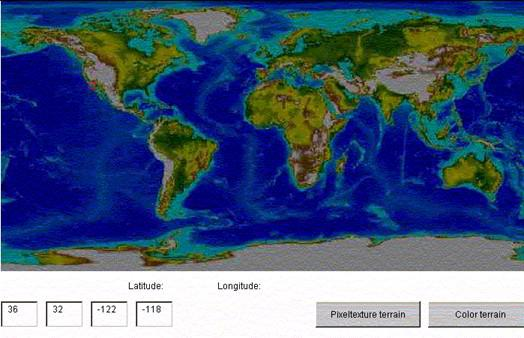
\includegraphics[width=0.4\textwidth]{WebGrafikleri.jpg}
\caption{web grafikleri}
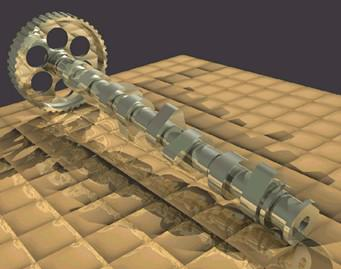
\includegraphics[width=0.3\textwidth]{CAD.jpg}
\caption{CAD}
\end{figure}
\end{frame}

\begin{frame}{Diğer Kullanım Alanları}
\begin{figure}
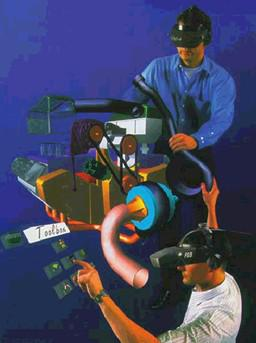
\includegraphics[width=0.2\textwidth]{SanalGerçeklik.jpg}
\caption{Sanal Gerçeklik}
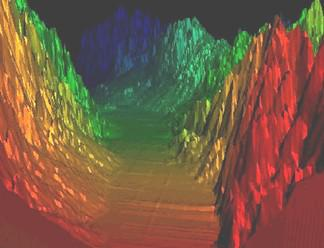
\includegraphics[width=0.3\textwidth]{bilimsel vizualasyon.jpg}
\caption{Bilimsel vizualasyon}
\end{figure}
\end{frame}

\begin{frame}{OpenGL'de Örnek Bir Üçgen Çizimi}
\lstinputlisting{codes/section1.cpp}
\end{frame}

\begin{frame}{OpenGL'de Örnek Bir Üçgen Çizimi}
\lstinputlisting{codes/section2.cpp}
\end{frame}

\begin{frame}{OpenGL'de Örnek Bir Üçgen Çizimi}
\lstinputlisting{codes/section3.cpp}
\end{frame}

\begin{frame}{OpenGL'de Örnek Bir Üçgen Çizimi}
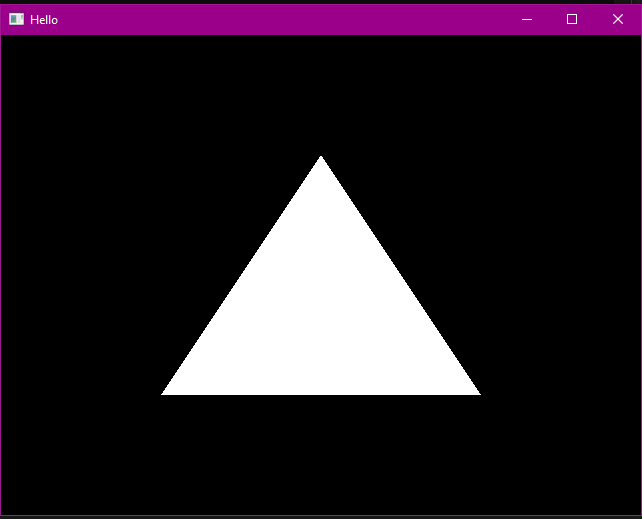
\includegraphics[width=0.5\textwidth]{backgrounds/triangle.png}
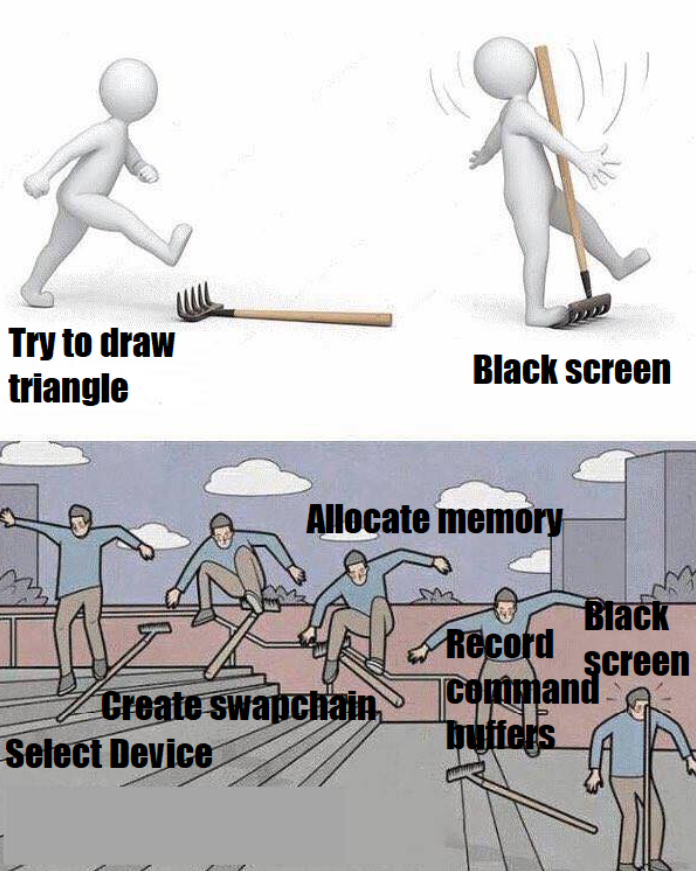
\includegraphics[width=0.4\textwidth]{ouch.png}
\caption{}
\end{frame}




% [allowframebreaks] özelliği eğer sayfadaki metin 1 sayfayı aşarsa otomatik sayfalara bölmeyi sağlar
\begin{frame}[allowframebreaks]{Kaynaklar}
  \bibliographystyle{plain}
  \scriptsize
  \bibliography{kaynak}
\end{frame}

\end{document}